\documentclass[10pt]{article}
\setlength{\parskip}{\baselineskip}
\usepackage{fullpage}
\usepackage[margin = 0.5in]{geometry}
\usepackage{multirow}
\usepackage{csquotes}
\usepackage{graphicx}
\usepackage{amsmath,amsfonts,amssymb}
\usepackage{array}
\usepackage[table]{xcolor}

\title{Homework 3}
\author{CSCI 4511W Spring 2018}
\begin{document}
\date{March 21, 2018}
\maketitle

Instructor: Dr.Maria Gini\hfill Joowon Kim(kimx4342)

\hrulefill

\begin{enumerate}
\item Decide if the following sentences are valid, unsatisfiable, or neither. To do it, use the truth tables and equivalency rules in Chapter 7.
  \begin{enumerate}
  \item Big $\Rightarrow$ Big \par
  \fbox{$\rightarrow$ Valid} 
  \begin{displaymath}
    \begin{array} {|c|c|c|}
  	  \hline
      Big & Big & Big \Rightarrow Big \\
      \hline
      True & True & \cellcolor{gray!25}True\\
      False & False & \cellcolor{gray!25}True\\
      \hline
    \end{array}
  \end{displaymath}
  \item Big $\Rightarrow$ Heavy \par
  \fbox{$\rightarrow$ Neither (satisfiable)}
   \begin{displaymath}
    \begin{array} {|c|c|c|}
  	  \hline
      Big & Heavy & Big \Rightarrow Heavy \\
      \hline
      True & True & \cellcolor{gray!25}True \\
      True & False & \cellcolor{gray!25}False \\
      False & True & \cellcolor{gray!25}True \\
      False & False & \cellcolor{gray!25}True \\
      \hline
    \end{array}
  \end{displaymath}
  \item (Big $\Rightarrow$ Heavy) $\Rightarrow$ ($\neg$ Big $\Rightarrow$ $\neg$ Heavy) \par
  \fbox{$\rightarrow$ Neither (satisfiable)}
   \begin{displaymath}
    \begin{array} {|c|c|c|c|c|c|}
  	  \hline
      Big & Heavy & \neg Big & \neg Heavy & Big \Rightarrow Heavy & \neg Big \Rightarrow \neg Heavy \\
      \hline
      True & True & False & False & True & True \\
      True & False & False & True & False & True  \\
      False & True & True & False & True & False \\
      False & False & True & True & True & True \\
      \hline\hline
      \multicolumn{6}{|c|}{(Big \Rightarrow Heavy) \Rightarrow (\neg Big \Rightarrow \neg Heavy)}\\
      \hline
      \multicolumn{6}{|c|}{\cellcolor{gray!25}True} \\
      \multicolumn{6}{|c|}{\cellcolor{gray!25}True} \\
      \multicolumn{6}{|c|}{\cellcolor{gray!25}False} \\
      \multicolumn{6}{|c|}{\cellcolor{gray!25}True} \\
      \hline
    \end{array}
  \end{displaymath}
  \item Big $\vee$ Heavy $\vee$ $\neg$ Heavy \par
  \fbox{$\rightarrow$ Valid}
  \begin{displaymath}
    \begin{array} {|c|c|c|c|}
  	  \hline
      Big & Heavy & \neg Heavy & Big \vee Heavy \vee \neg Heavy \\
      \hline
      True & True & False & \cellcolor{gray!25}True \\
      True & False & True & \cellcolor{gray!25}True \\
      False & True & False & \cellcolor{gray!25}True \\
      False & False & True & \cellcolor{gray!25}True \\
      \hline
    \end{array}
  \end{displaymath}
  \newpage
  \item ((Big $\wedge$ Dense) $\Rightarrow$ Heavy) $\Leftrightarrow$ ((Big $\Rightarrow$ Dense) $\vee$ (Heavy $\Rightarrow$ Dense)) \par
  \fbox{$\rightarrow$ Neither (satisfiable)}
  \begin{displaymath}
    \begin{array} {|c|c|c|c|c|c|c|c|}
  	  \hline
      Big & Dense & Heavy & Big \wedge Dense & Big \Rightarrow Dense & Heavy \Rightarrow Dense & (Big \wedge Dense) \Rightarrow Heavy \\
      \hline
      True & True & True & True & True & True & True  \\
      True & True & False & True & True & True & False \\
      True & False & True & False & False & False & True \\
      True & False & False & False & False & True & True \\
      False & True & True & False & True & True & True \\
      False & True & False & False & True & True & True \\
      False & False & True & False & True & False & True \\
      False & False & False & False & True & True & True \\
      \hline\hline
      \multicolumn{3}{|c|}{(Big \Rightarrow Dense) \vee (Heavy \Rightarrow Dense)} & \multicolumn{4}{c|}{((Big \wedge Dense) \Rightarrow Heavy) \Leftrightarrow ((Big \Rightarrow Dense) \vee (Heavy \Rightarrow Dense))} \\
      \hline
     \multicolumn{3}{|c|}{True} & \multicolumn{4}{c|}{\cellcolor{gray!25}True}\\
     \multicolumn{3}{|c|}{True} & \multicolumn{4}{c|}{\cellcolor{gray!25}False}\\
     \multicolumn{3}{|c|}{False} & \multicolumn{4}{c|}{\cellcolor{gray!25}False}\\
     \multicolumn{3}{|c|}{True} & \multicolumn{4}{c|}{\cellcolor{gray!25}True}\\
     \multicolumn{3}{|c|}{True} & \multicolumn{4}{c|}{\cellcolor{gray!25}True}\\
     \multicolumn{3}{|c|}{True} & \multicolumn{4}{c|}{\cellcolor{gray!25}True}\\
     \multicolumn{3}{|c|}{True} & \multicolumn{4}{c|}{\cellcolor{gray!25}True}\\
     \multicolumn{3}{|c|}{True} & \multicolumn{4}{c|}{\cellcolor{gray!25}True}\\
     \hline
    \end{array}
  \end{displaymath}
  \item (Big $\Rightarrow$ Dense) $\Rightarrow$ ((Big $\wedge$ Heavy) $\Rightarrow$ Dense) \par
  \fbox{$\rightarrow$ Valid}
  \begin{displaymath}
    \begin{array} {|c|c|c|c|c|c|}
  	  \hline
      Big & Heavy & Dense & Big \Rightarrow Dense & Big \wedge Heavy & (Big \wedge Heavy) \Rightarrow Dense \\
      \hline
      True & True & True & True & True & True \\
      True & True & False & False & True & False \\
      True & False & True & True & False & True  \\
      True & False & False & False & False & True \\
      False & True & True & True & False & True  \\
      False & True & False & True & False & True \\
      False & False & True & True & False & True \\
      False & False & False & True & False & True \\
      \hline\hline
      \multicolumn{6}{|c|}{(Big \Rightarrow Dense) \Rightarrow ((Big \wedge Heavy) \Rightarrow Dense)} \\
      \hline
      \multicolumn{6}{|c|}{\cellcolor{gray!25}True} \\
      \multicolumn{6}{|c|}{\cellcolor{gray!25}True} \\
      \multicolumn{6}{|c|}{\cellcolor{gray!25}True} \\
      \multicolumn{6}{|c|}{\cellcolor{gray!25}True} \\
      \multicolumn{6}{|c|}{\cellcolor{gray!25}True} \\
      \multicolumn{6}{|c|}{\cellcolor{gray!25}True} \\
      \multicolumn{6}{|c|}{\cellcolor{gray!25}True} \\
      \multicolumn{6}{|c|}{\cellcolor{gray!25}True} \\
      \hline
    \end{array}
  \end{displaymath}
  \item Small $\vee$ Cute $\vee$ (Small $\Rightarrow$ Cute) \par
  \fbox{$\rightarrow$ Valid}
  \begin{displaymath}
    \begin{array} {|c|c|c|c|}
  	  \hline
      Small & Cute & Small \Rightarrow Cute & Small \vee Cute \vee (Small \Rightarrow Cute) \\
      \hline
      True & True & True & \cellcolor{gray!25}True \\
      True & False & False & \cellcolor{gray!25}True \\
      False & True & True & \cellcolor{gray!25}True \\
      False & False & True & \cellcolor{gray!25}True \\
      \hline
    \end{array}
  \end{displaymath}
  \item (Small$\wedge$ Cute) $\vee$ $\neg$ Cute \par
 \fbox{$\rightarrow$ Neither (satisfiable)}
  \begin{displaymath}
    \begin{array} {|c|c|c|c|c|}
  	  \hline
      Small & Cute & \neg Cute & Small \wedge Cute & (Small \wedge Cute) \vee \neg Cute \\
      \hline
      True & True & False & True & \cellcolor{gray!25}True \\
      True & False & True & False & \cellcolor{gray!25}True \\
      False & True & False & False & \cellcolor{gray!25}False \\
      False & False & True & False & \cellcolor{gray!25}True \\
      \hline
    \end{array}
  \end{displaymath}
  \item ((Rain $\Rightarrow$ Wet) $\wedge$ (Wet $\Rightarrow$ Cold)) $\Rightarrow$ (Rain $\Rightarrow$ Cold) \par
  \fbox{$\rightarrow$ Valid}
  \begin{displaymath}
    \begin{array} {|c|c|c|c|c|c|c|}
  	  \hline
      Rain & Wet & Cold & Rain \Rightarrow Wet & Wet \Rightarrow Cold & Rain \Rightarrow Cold & (Rain \Rightarrow Wet) \wedge (Wet \Rightarrow Cold) \\
      \hline
      True & True & True & True & True & True & True  \\
      True & True & False & True & False & False & False \\
      True & False & True & False & True & True & False \\
      True & False & False & False & True & False & False \\
      False & True & True & True & True & True & True  \\
      False & True & False & True & False & True & False  \\
      False & False & True & True & True & True & True \\
      False & False & False & True & True & True & True \\
      \hline\hline
      \multicolumn{7}{|c|}{((Rain \Rightarrow Wet) \wedge (Wet \Rightarrow Cold)) \Rightarrow (Rain \Rightarrow Cold)} \\
      \hline
      \multicolumn{7}{|c|}{\cellcolor{gray!25}True} \\
      \multicolumn{7}{|c|}{\cellcolor{gray!25}True} \\
      \multicolumn{7}{|c|}{\cellcolor{gray!25}True} \\
      \multicolumn{7}{|c|}{\cellcolor{gray!25}True} \\
      \multicolumn{7}{|c|}{\cellcolor{gray!25}True} \\
      \multicolumn{7}{|c|}{\cellcolor{gray!25}True} \\
      \multicolumn{7}{|c|}{\cellcolor{gray!25}True} \\
      \multicolumn{7}{|c|}{\cellcolor{gray!25}True} \\
      \hline
    \end{array}
  \end{displaymath}
  \item ((Rain $\vee$ Wet) $\wedge$ ($\neg$ Wet $\vee$ Cold)) $\Rightarrow$ (Rain $\vee$ Cold) \par
  \fbox{$\rightarrow$ Valid}
  \begin{displaymath}
    \begin{array} {|c|c|c|c|c|c|c|}
  	  \hline
      Rain & Wet & Cold & \neg Wet & Rain \vee Wet & \neg Wet \vee Cold & Rain \vee Cold \\
      \hline
      True & True & True & False & True & True & True \\
      True & True & False & True & True & True & True \\
      True & False & True & True & True & True & True \\
      True & False & False & True & True & True & True \\
      False & True & True & False & True & True & True \\
      False & True & False & False & True & False & False \\
      False & False & True & True & False & True & True \\
      False & False & False & True & False & True & False \\
      \hline\hline
      \multicolumn{2}{|c|}{(Rain \vee Wet) \wedge (\neg Wet \vee Cold)} & \multicolumn{5}{c|}{((Rain \vee Wet) \wedge (\neg Wet \vee Cold)) \Rightarrow (Rain \vee Cold)} \\
      \hline
      \multicolumn{2}{|c|}{True} & \multicolumn{5}{c|}{\cellcolor{gray!25}True}\\
      \multicolumn{2}{|c|}{True} & \multicolumn{5}{c|}{\cellcolor{gray!25}True}\\
      \multicolumn{2}{|c|}{True} & \multicolumn{5}{c|}{\cellcolor{gray!25}True}\\
      \multicolumn{2}{|c|}{True} & \multicolumn{5}{c|}{\cellcolor{gray!25}True}\\
      \multicolumn{2}{|c|}{True} & \multicolumn{5}{c|}{\cellcolor{gray!25}True}\\
      \multicolumn{2}{|c|}{False} & \multicolumn{5}{c|}{\cellcolor{gray!25}True}\\
      \multicolumn{2}{|c|}{False} & \multicolumn{5}{c|}{\cellcolor{gray!25}True}\\
      \multicolumn{2}{|c|}{False} & \multicolumn{5}{c|}{\cellcolor{gray!25}True}\\
      \hline
    \end{array}
  \end{displaymath}
  \end{enumerate}
  \newpage
\item For each of the following formulas, state briefly if it is a correct representation in propositional calculus of the sentence "If Bill works and his father stays at home, then his mother is happy" or not and explain why. The propositions used in the sentences should have an obvious interpretation. \par
$\Rightarrow$ Possible propositional calculus of "If Bill works and his father stays at home, then his mother is happy" is \par
(BillWork $\wedge$ DadHome) $\Rightarrow$ MomHappy \par
$\equiv$ $\neg$ (BillWork $\wedge$ DadHome) $\vee$ MomHappy [Implication Elimination] \par
$\equiv$ ($\neg$ BillWork $\vee$ $\neg$ DadHome) $\vee$ MomHappy [De Morgan] \par
$\equiv$ $\neg$ MomHappy $\Rightarrow$ $\neg$ (BillWork $\wedge$ DadHome) [Contraposition]
  \begin{enumerate}
  \item BillWork $\wedge$ DadHome $\wedge$ MomHappy \par
  $\rightarrow$ This is an \fbox{incorrect} representation. It says BillWork and DadHome and MomHappy and implies the conjunction of MomHappy, which should not.
  \item (BillWork $\wedge$ DadHome) $\Rightarrow$ MomHappy \par
  $\rightarrow$ This is a \fbox{correct} representation by the Implication Elimination I wrote above.
  \item (BillWork $\vee$ DadHome) $\Rightarrow$ MomHappy \par
  $\rightarrow$ This is an \fbox{incorrect} representation. It does not represent the conjunction of BillWork and DadHome.
  \item MomHappy $\Rightarrow$ (BillWork $\wedge$ DadHome) \par
  $\rightarrow$ This is an \fbox{incorrect} representation. If both sides are negated, than it would be a correct sentence by contraposition. 
  \item $\neg$ BillWork $\vee$ ($\neg$ MomHappy $\vee$ DadHome) \par
  $\rightarrow$ This is an \fbox{incorrect} representation. If MomHappy is not negated and instead, DadHome is negated, than it would be a correct sentence by De Morgan.
  \end{enumerate}

\item  Convert the following set of propositional clauses to CNF and prove by resolution with refutation that it is Pleasant.
  \begin{enumerate}
  \item Cold $\wedge$ Dry $\Rightarrow$ Pleasant \par
  $\equiv$ $\neg$ (Cold $\wedge$ Dry) $\vee$ Pleasant [Implication Elimination] \par
  $\equiv$ $\neg$ Cold $\vee$ $\neg$ Dry $\vee$ Pleasant [De Morgan]
  \item January $\Rightarrow$ Winter $\wedge$ Wet \par
  $\equiv$ $\neg$ January $\vee$ (Winter $\wedge$ Wet) [Implication Elimination] \par
  $\equiv$ ($\neg$ January $\vee$ Winter) $\wedge$ ($\neg$ January $\vee$ Wet) [Distributivity]
  \item Winter $\Rightarrow$ Dry \par
  $\equiv$ $\neg$ Winter $\vee$ Dry [Implication Elimination]
  \item Wet $\Rightarrow$ Cold \par
  $\equiv$ $\neg$ Wet $\vee$ Cold [Implication Elimination]
  \item January
  \end{enumerate}
  $\rightarrow$ \par
  \begin{center}
  January, $\neg$ January $\vee$ (Winter $\wedge$ Wet) \par 
  \hrulefill
  
  \textbf{(Winter $\wedge$ Wet) $\equiv$ $\neg$ Winter $\vee$ $\neg$ Wet} \par
  $\neg$ Winter $\vee$ $\neg$ Wet , $\neg$ Wet $\vee$ Cold \par
  \hrulefill
  
  \textbf{$\neg$ Winter $\vee$ $\neg$ Wet $\vee$ Cold} \par
  $\neg$ Cold $\vee$ $\neg$ Dry $\vee$ Pleasant , $\neg$ Winter $\vee$ Dry \par
  \hrulefill
  
  \textbf{$\neg$ Winter $\vee$ $\neg$ Cold $\vee$ Pleasant} \par
  $\neg$ Winter $\vee$ $\neg$ Cold $\vee$ Pleasant , $\neg$ Winter $\vee$ $\neg$ Wet $\vee$ Cold \par
  \hrulefill
  
  \textbf{$\neg$ Winter $\vee$ $\neg$ Wet $\vee$ pleasant} \par
  \textbf{$\equiv$ $\neg$ (Winter $\wedge$ Wet) $\vee$ Pleasant} [De Morgan] \par
  \textbf{$\equiv$ (Winter $\wedge$ Wet) $\Rightarrow$ Pleasant} [Implication Elimination]
  \end{center}
\newpage

\item Programming questions.
	\begin{enumerate}
		\item Create a propositional data base, include in it the clauses from problem 3 above and prove it is Pleasant using the program.
        \item Create a propositional data base and represent the following: \enquote{If the unicorn is mythical, then it is immortal but if it is not mythical then it is a mortal mammal. If the unicorn is either immortal or a mammal, then it is horned. The unicorn is magical, if it is horned.}
        \item Use ask to answer the following questions from the data base you created for the previous question: 
        \begin{enumerate}
        \item is the unicorn mythical?
        \item is the unicorn magical?
        \item is the unicorn horned?
        \end{enumerate}
        What can you say from the answers you get? Do the statements logically follow from the knowledge base? or not? \newline
        $\rightarrow$ The output of the program is attached, as well the code I modified. \newline
	\end{enumerate}
    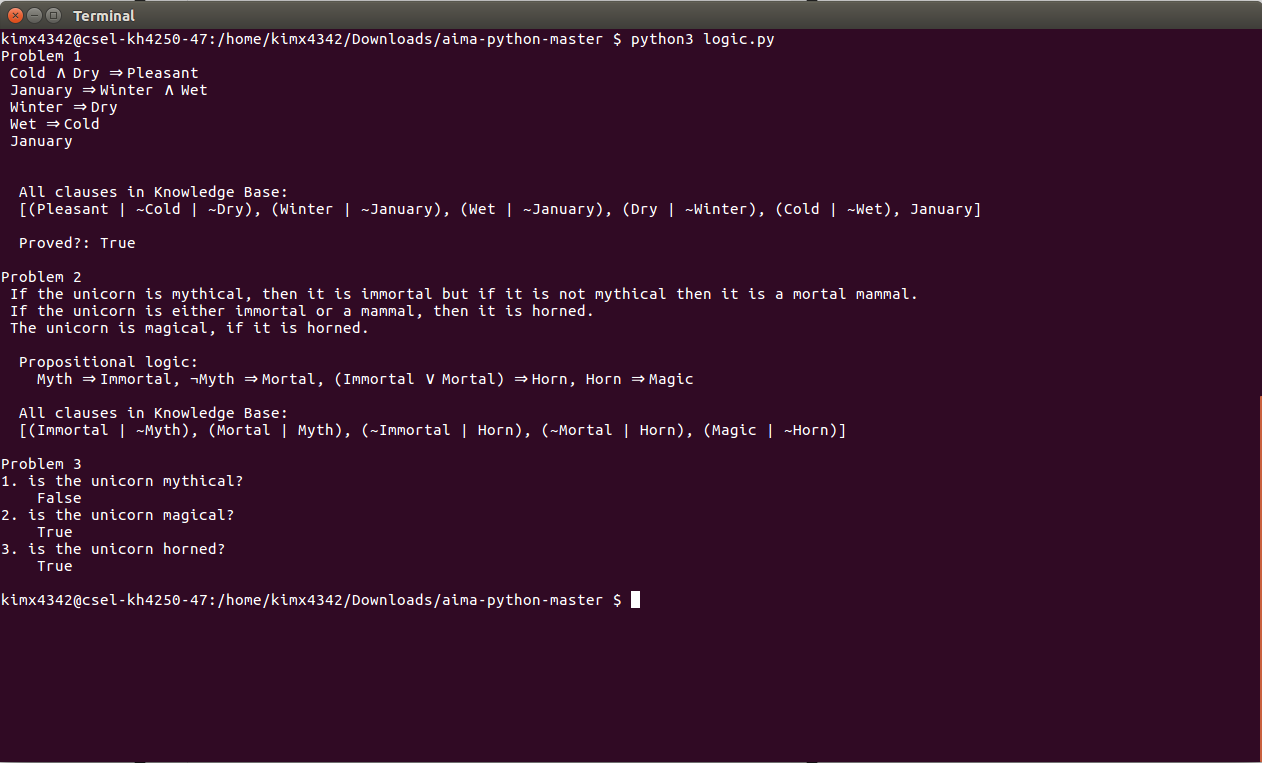
\includegraphics[width=\textwidth]{hw3_1.png}
    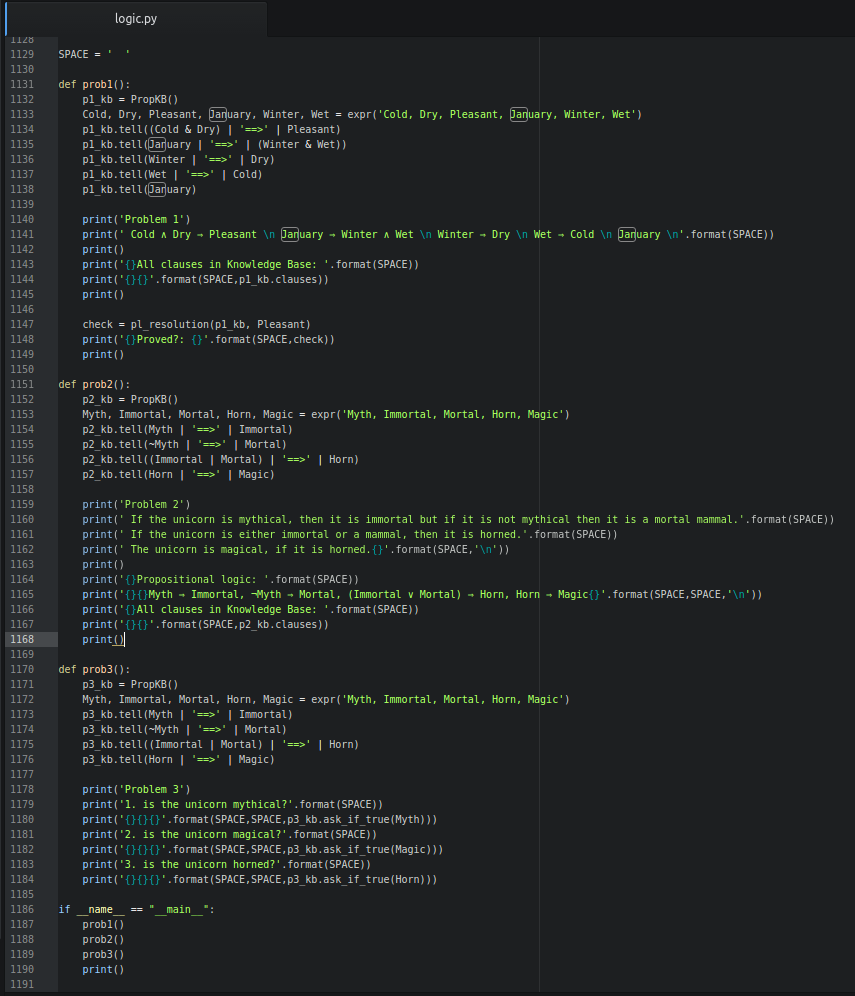
\includegraphics[width=\textwidth]{hw3code1.png}
\end{enumerate}

\end{document}